\documentclass[final]{beamer}
  \mode<presentation>
  {
% you can chose your theme here:
%  \usetheme{Aachen}
  \usetheme{I6dv}
%  \usetheme{I6pd}
%      \usetheme{Berlin}
%  \usetheme{I6pd2}
%  \usetheme{I6td}
%  \usetheme{Oldi6}
}
%\graphicspath{{figures/}}

\usepackage{setspace} 
\usepackage{wrapfig}
\usepackage[numbers, compress]{natbib}

\usepackage{graphicx}

\usepackage{subcaption}
\usepackage{lipsum}
\usepackage{times}
\usepackage{booktabs}       % professional-quality tables

\usepackage{makecell}
\usepackage{blindtext}
\usepackage{amsmath,amssymb}
\usepackage{booktabs, array}
\usepackage{algorithm}
\usepackage{algorithmic}
\usepackage{dsfont}
\usepackage{wasysym}
\usepackage{fancybox}
\usepackage[english]{babel}
\usepackage[latin1]{inputenc}
\usepackage{mathtools}
\usepackage[orientation=portrait,size=a0,scale=1]
{beamerposter}  % e.g. custom size poster
  \title{{Toward Bayesian permutation inference for identifying neurons in \textit{C. elegans}.}}
  \author[]{Gonzalo E. Mena$^{1,*}$, Scott Linderman $^{1,*}$, David Belanger $^2$, Jasper Snoek $^2$, John Cunningham$^{1,3}$, Liam Paninski$^{1,3}$}
  \institute[]{\linebreak 1. Department of Statistics, Columbia University, New York, NY, USA 2. Google Brain, Cambridge, MA.
   3. Center for Theoretical Neuroscience and Grossman Center for the Statistics of Mind, Columbia University, New York, NY, USA.}

\newcommand{\logit}{\text{logit}}
\newcommand{\Bernoulli}{\text{Bernoulli}}
\newcommand{\N}{\mathcal{N}}
\newcommand{\p}{\text{p}}
\newcommand{\bfx}{\mathbf{x}}
\newcommand{\bfy}{\mathbf{y}}
\newcommand{\bfm}{\mathbf{m}}
\newcommand{\bfb}{\mathbf{b}}
\newcommand{\bfh}{\mathbf{h}}
\newcommand{\bfd}{\mathbf{d}}




\makeatletter
    \newenvironment{withoutheadline}{
        \setbeamertemplate{headline}[default]
        \def\beamer@entrycode{\vspace*{-\headheight}}
    }{}
\makeatother


\begin{document}

 \begin{frame}[allowframebreaks]

     \begin{minipage}[htp][1\textheight][t]{\textwidth}

        \begin{columns}[t]
             \hspace{1cm} 
            \begin{column}{.5\linewidth}
              \begin{block}{Summary}
                        
	               \textbf{Overarching goal}
	               \large
              		\begin{itemize}
		\item State and infer Bayesian hierarchical models for the activity in C.elegans	combining information (calcium traces) from several worms.   
		\item This is possible as C.elegans nervous system is stereotypical, neurons and connectome don't change across individuals.
		 \end{itemize}
		 	 \textbf{Challenge}
              		\begin{itemize}
		\item If neural identity is known for each trace, one can apply standard bayesian methodology
		\item In practice, laborious human supervision is needed to match recorded traces to canonical neural identities (i.e. names) \end{itemize}

		\textbf{Our contribution}
	\begin{itemize}
	\item We developed three methods for learning latent matchings. These can be used in variational inference (VI) to jointly estimate a dynamical system and the matching between traces and true neural identities.
	\item Potentially it may serve to automatize the matching procedure.
	\item From a statistical machine learning perspective, the relevance is that outperforms a simple MCMC sampler for permutations.
	\end{itemize}
	\textbf{Future work}
	\begin{itemize}
	\item We used real connectome a position information. In the future we plan to use real traces.
	\item Two new levels of complexity: partially observed brain recordings, more sophisticated dynamical systems.
	\end{itemize}
	   
	 
	    \end{block}
	    
\begin{block}{Model}
\large Simple linear autoregressive
model for neural dynamics,
\begin{align}
  \widetilde{Y}_t^{(j)} &= (W \odot A) \widetilde{Y}_{t-1}^{(j)} + \epsilon_t^{(j)},
\end{align}
where~$W \in \mathbb{R}^{N \times N}$ is the weight matrix (gaussian prior);
$A \in \{0,1\}^{N \times N}$ is the connectome;
$\epsilon_t^{(j)} \sim \mathcal{N}(0, \sigma^2 I)$;
and~$\widetilde{Y}_t^{(j)} \in \mathbb{R}^N$ is the measured neural activity
at time~$t$ in worm~$j$.  The catch is that~$\widetilde{Y}_t^{(j)}$ is
assumed to be in canonical order; i.e. in the same order as the rows and
columns of~$W$ and~$A$. We actually observe,
\begin{align}
  Y_t^{(j)} &= P^{(j)} \widetilde{Y}_t^{(j)}.
\end{align}
We aim to perform posterior inference of $p(\{W,P^{(j)}\} \, | \, A, \{Y^{(j)}\})$.
\vspace{0.5cm}

The permutations are constrained by side
information: we use neural position along the worm's
body to constrain the possible neural identities for a given recorded
neuron. We only allow an observed neuron to be mapped to a known
identity if the observed location is within~$\eta$ of the expected
location.  

\end{block}

	 	             	    
\begin{block}{Experimental setup}

\begin{figure}[t]
  \centering
  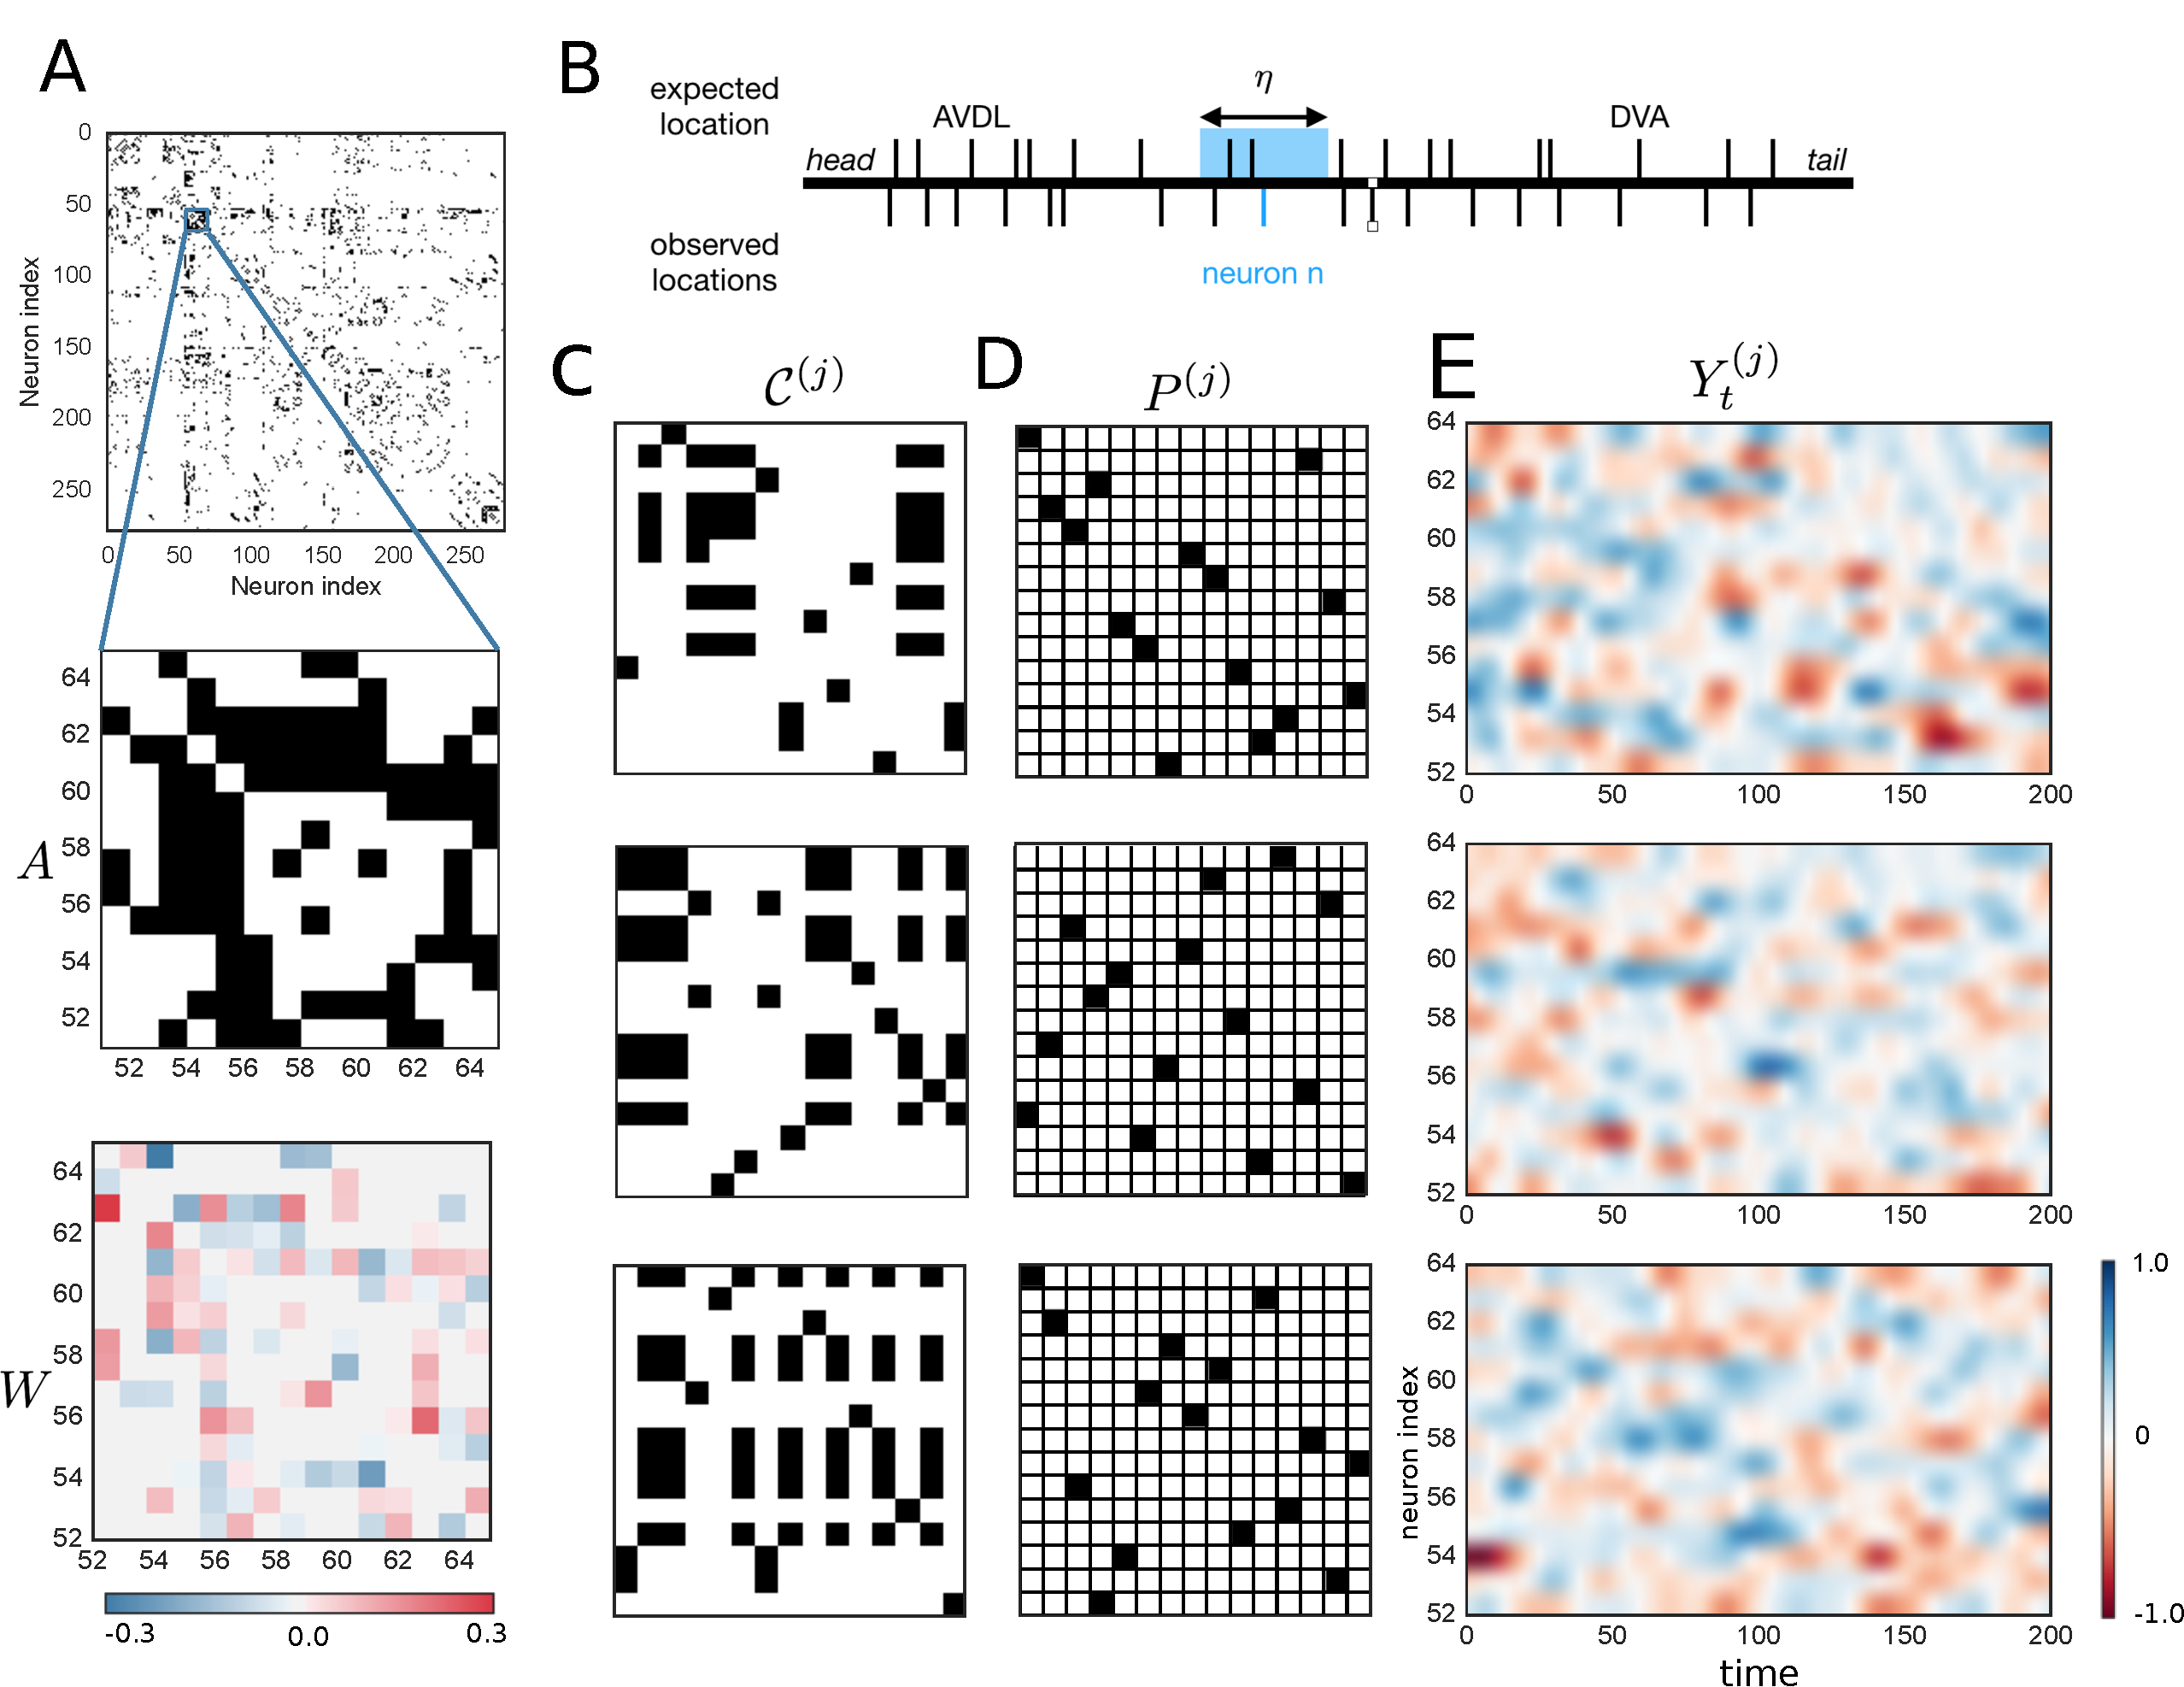
\includegraphics[width=0.7\textwidth]{figs/Figure3.pdf} 
  \caption\large {\textit{Hierarchical Bayesian framework}.  \textbf{A} Adjacency matrix (connectome) $A$ from
    \cite{varshney2011structural}.  We wish to infer the
    corresponding weight matrix~$W$. \textbf{B} We know the typical locations of the
    neurons \cite{white1986structure,wormatlas}. 
    We constrain possible assignments to neuron identities
    within~$\eta$ of the observed location.  \textbf{C} These
    constraints are represented as a matrix $\mathcal{C}^{(j)}$ for
    worm~$j$ specifying possible assignments of observed neurons
    to identities.     \textbf{D} To infer the weights, we must first infer the
    permutation $P^{(j)}$ that matching observed neurons to the set of known identities.  \textbf{E} The observed
    data is a matrix~$Y^{(j)}$  with non-canonical order. }

\label{fig:1}
\end{figure}



	   \end{block}
   	
	
	  \begin{block}{Three reparameterizations for permutations}
\large  We extend to permutations the \emph{Concrete} or \emph{Gumbel softmax} relaxations \cite{Jang2016,Maddison2016} in three different ways. In all relaxations we are concerned with $\mathcal{B}_N$, the Birkhoff polytope or set of doubly-stochastic matrices. 
	  \end{block}
            \end{column}    


            
            \begin{column}{.5\linewidth}
           
	              
	  
	    \begin{block}{Stick-Breaking and Rounding}
	    \large
	    On the stick-breaking we generalize the construction on the simplex \cite{linderman2015dependent} to
$\mathcal{B}_N$. For the
rounding construction, we start with a noise distribution and force it
to be close to permutation matrices by rounding them towards the
extreme-points of $\mathcal{B}_N$.
           	 \begin{figure}
	    	\centering
		{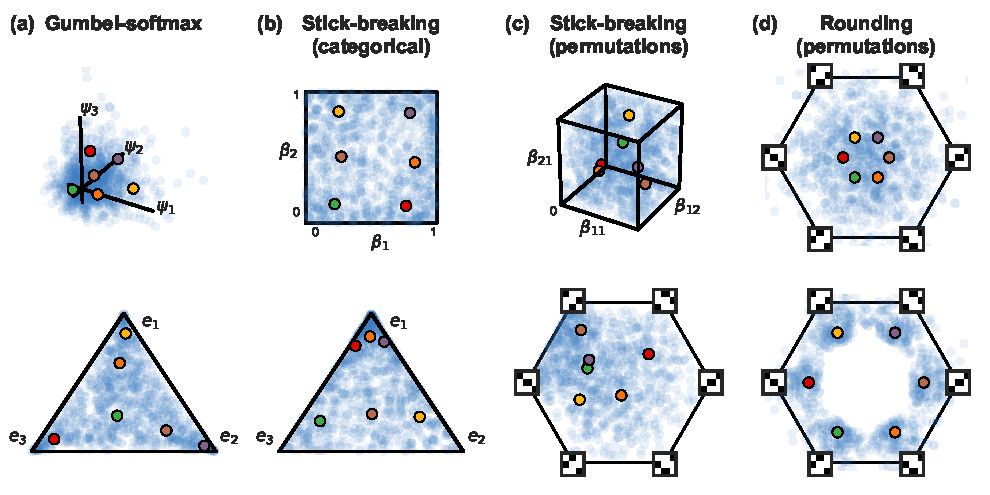
\includegraphics[width=1.0\textwidth]{figs/Figure1.pdf}}
		 \caption{\normalsize Rounding and Stick-breaking transformations of noise, and relation to constructions in the simplex }
\label{fig:transforms}
	\end{figure}


	  
\end{block}
	
	     
	\begin{block}{Gumbel-Sinkhorn ($\mathcal{G.S}$) distribution}
	\large
We use the \emph{Sinkhorn operator} $S(\cdot)$, the successive row and
column normalization of a matrix. This approximates the choice of a permutation $M(X)$; i.e. $M(X)=\lim_{\tau\rightarrow 0} S(X/\tau)$. By adding Gumbel noise we conceive the Gumbel Matching distribution and its approximation, the  \emph{G.S.} distribution.
			\begin{figure}
         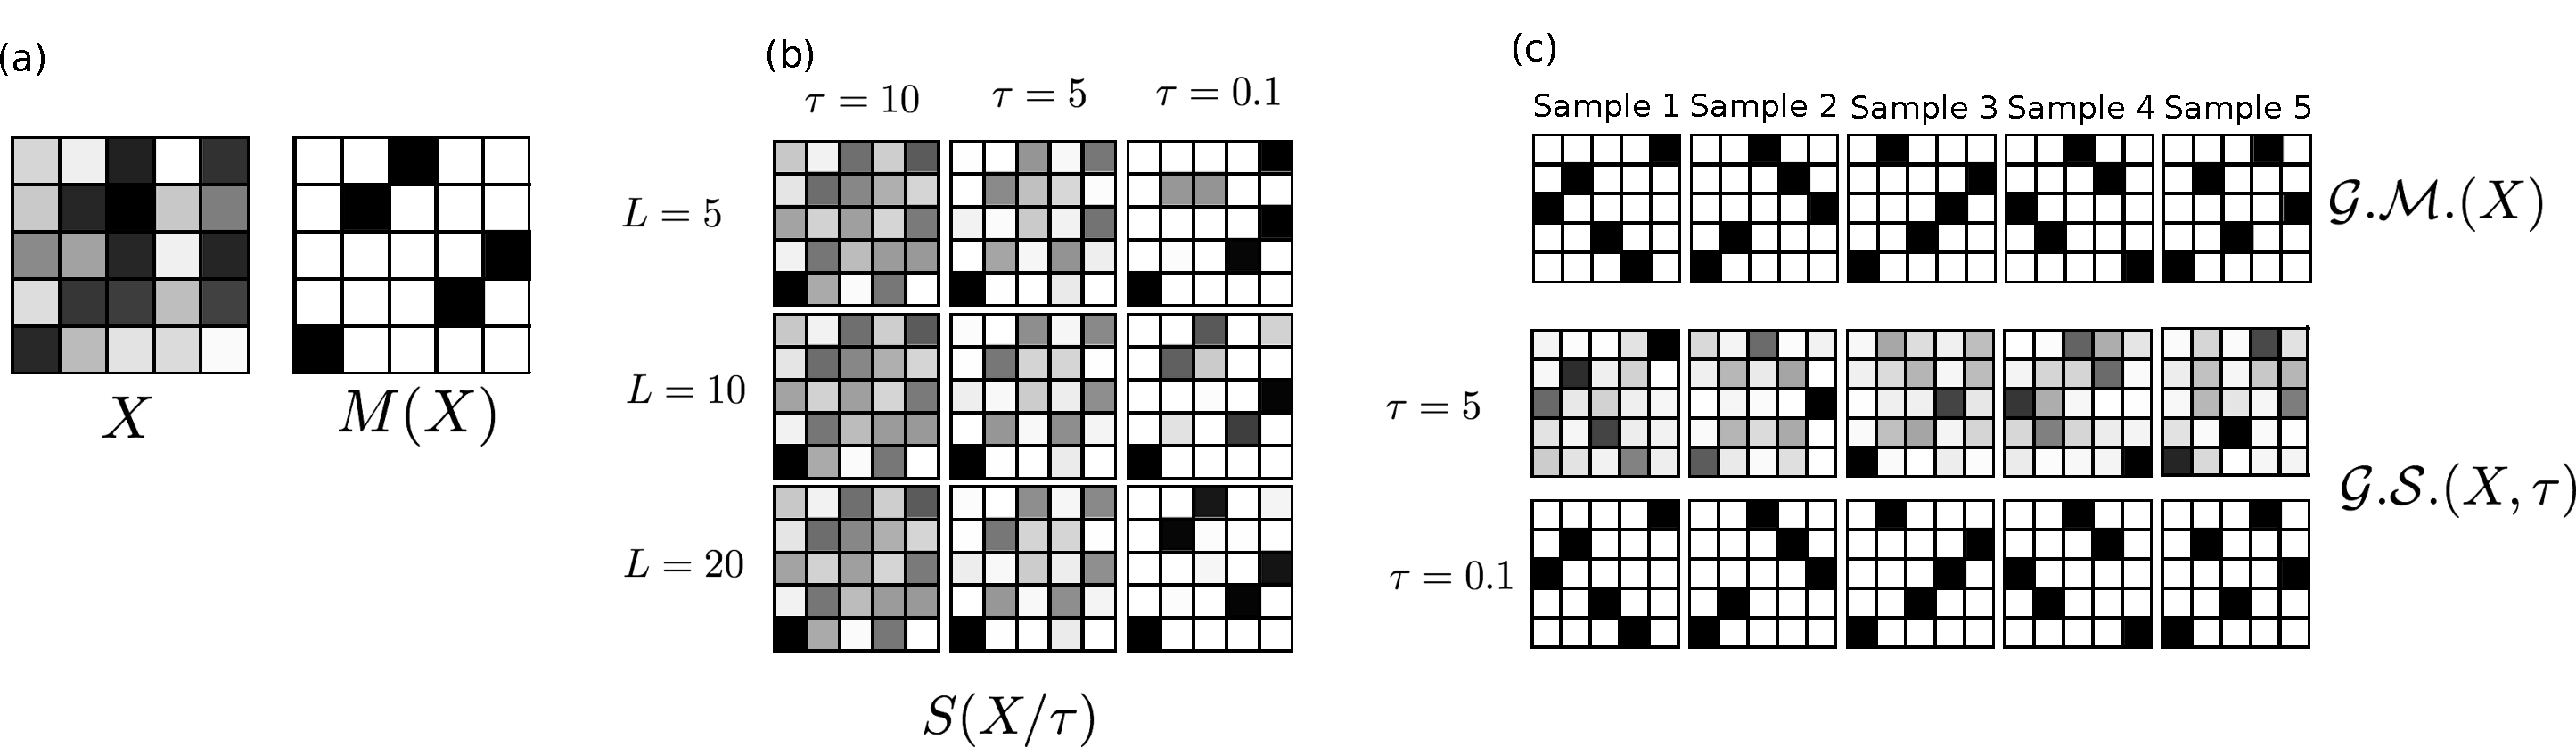
\includegraphics[trim = 0cm 0cm 0mm 0.0cm, clip=true, width=1.0\textwidth]{figs/Figure2.pdf}
	 \caption{\normalsize Matching and Sinkhorn operators, and the Gumbel-Matching and Gumbel-Sinkhorn distributions.}
 \label{fig:figure2}
 \end{figure} 
            \end{block}	
             

      	\begin{block}{Results}
	\large
We compared against: (i) na\"ive variational inference,
where we do not enforce the constraint that $P^{(j)}$ be a permutation; (ii) MCMC, where we alternate between sampling from the
conditionals of $W$ (Gaussian) and ${P^{(j)}}$, from which one can
sample by proposing local swaps, as described in \cite{Diaconis2009},
and (iii) MAP estimation. 


\begin{table}[t]
     \caption{Accuracy in the C.elegans neural identification problem, for varying mean number of candidate neurons (10, 30, 45, 60) and number of worms.}
   \label{table:celeganssup}

   \centering
  \begin{tabular}{lllllllllll}
    & \multicolumn{2}{c}{10} & \multicolumn{2}{c}{30} &   \multicolumn{2}{c}{45} & \multicolumn{2}{c}{60} \\
    \cmidrule(lr){2-3} \cmidrule(lr){4-5} \cmidrule(lr){6-7} \cmidrule(lr){8-9}
& 1 worm & 4 worms & 1 Worm & 4 worms & 1 worm & 4 worms & 1 worms & 4 worms \\
    \midrule 
    NAIVE VI &.34 & .32 & .16 & .16 & .13 & .12 & .11 & .12 \\
   MAP   & .34 & .32  &.17 &.17& .14 & .13 & .13 & .12 \\
    MCMC   & .34 & .65  &.18 &.28& .14 & .17 & .13 & .15 \\
  
    VI   & \textbf{.79} & \textbf{.94} & \textbf{.4} & \textbf{.69} & \textbf{.25}&  \textbf{.51} & \textbf{.21} & \textbf{.44}\\
 
    \bottomrule
  \end{tabular}
\end{table}


\begin{table}[t]
  \caption{Accuracy in inferring true neural identity for different of
    proportion of known neurons and $\eta$.
  }
   \label{table:celegans}
   \centering
   \begin{tabular}{lllllllll}
    & \multicolumn{2}{c}{40.\%} & \multicolumn{2}{c}{30.\%} & \multicolumn{2}{c}{20.\%} & \multicolumn{2}{c}{10.\%}\\
    \cmidrule(lr){2-3} \cmidrule(lr){4-5} \cmidrule(lr){6-7} \cmidrule(lr){8-9}
    & $\eta=0.1$ & $\eta=0.2$ & $\eta=0.1$ & $\eta=0.2$  & $\eta=0.1$ & $\eta=0.2$  & $\eta=0.1$ & $\eta=0.2$ \\
    \midrule 
    Naive VI & .43 & .41 & .33 & .31 & .23 & .22 & .12 & .1 \\
    MAP & .42 & .41  &.33 &.32& .23 & .22 & .12 & .11 \\
    MCMC   & .85 & .80  &.52 &.46& .3 & .26 & .15 & .12 \\
   %   \shortstack{Gumbel-Sinkhorn, no regularization (VI)} & .96 & .93 & .88 & .78 &  .69 & .52 & .39 & .21 \\
   %Rounding (VI)& \textbf{.97} & \textbf{.95} & \textbf{.90} & .84 & .75&  .\textbf{58} & \textbf{.37} & \textbf{.17} \\
    VI   & \textbf{.97} & \textbf{.96} & \textbf{.92} & \textbf{.84} & \textbf{.74} & \textbf{.58} & \textbf{.44} & \textbf{.23} \\
              \bottomrule
   \end{tabular}
\end{table}
\end{block}

   
	     \begin{block}{References}
	     \scriptsize
		\bibliography{refs}
\bibliographystyle{abbrvnat}


	\end{block}
	     	   		     

	     \end{column}
	     
            
            
            
	\end{columns}
      \end{minipage}
      
       
       

      
\end{frame}

\end{document}

%%%%%%%%%%%%%%%%%%%%%%%%%%%%%%%%%%%%%%%%%%%%%%%%%%%%%%%%%%%%%%%%%%%%%%%%%%%%%%%%%%%%%%%%%%%%%%%%%%%%
%%% Local Variables: 
%%% mode: latex
%%% TeX-PDF-mode: t